% IICTDS 2026 submission -- EAI single-column (Springer LNCS-style) format, 10-12 pages incl. references.
% Build:  cd paper && tectonic main.tex     (tables/ and figures/ are generated from results/:
%         python scripts/make_paper_tables.py && python scripts/make_paper_figures.py)
\documentclass[10pt,letterpaper]{article}
% ---- EAI CORE Proceedings template (EAI_Latex.tex v1.0, 2021-02-25) ----
\usepackage[top=5cm, bottom=5cm, left=3.8cm, right=3.8cm]{geometry}
\usepackage{mathptmx}
\usepackage{courier}
\usepackage{indentfirst}
\setlength{\parindent}{2.1em}
\usepackage{booktabs}
\usepackage{graphicx}
\usepackage[font=small,labelfont=bf]{caption}
\captionsetup[figure]{labelfont={bf},labelformat={default},labelsep=period,name={Fig.}}
\usepackage{titling}
\pretitle{\begin{center}\fontsize{16pt}{19pt}\selectfont\bfseries}
\posttitle{\par\end{center}\vskip 1ex}
\renewenvironment{abstract}{\begin{quote}\noindent {\small \bfseries \abstractname.} \small}{\medskip\noindent\end{quote}}
\newenvironment{keywords}{\begin{quote}\noindent {\small \bfseries Keywords: } \small}{\medskip\noindent\end{quote}}
\usepackage{titlesec}
\titleformat*{\section}{\large\bfseries}
\titleformat*{\subsection}{\normalsize\bfseries}
\titleformat*{\subsubsection}{\normalsize\bfseries}
\titleformat*{\paragraph}{\normalsize\bfseries}
\titleformat*{\subparagraph}{\normalsize\bfseries}
\renewcommand{\footnotesize}{\fontsize{9pt}{11pt}\selectfont}
\usepackage[hang,flushmargin]{footmisc}
% the template's bibspacing.sty: tighter bibliography item spacing
\let\oldthebibliography\thebibliography
\renewcommand{\thebibliography}[1]{\oldthebibliography{#1}\setlength{\itemsep}{.2\baselineskip plus .05\baselineskip minus .05\baselineskip}}
% ---- paper-specific ----
\usepackage{amsmath,amssymb,xcolor,url}
\usepackage[hidelinks]{hyperref}
\graphicspath{{figures/}}
\renewcommand{\topfraction}{0.9}\renewcommand{\bottomfraction}{0.8}\renewcommand{\textfraction}{0.07}\renewcommand{\floatpagefraction}{0.8}

\begin{document}

\title{On the Ring's Clock: Context-Aware Temporal Graph Neural Networks and Takedown-Value Training for Early Fraud-Ring Detection}

\author{
\normalsize First Author$^1$, Second Author$^1$ \\
\small $\lbrace$author1@institution.edu, author2@institution.edu$\rbrace$
\and
\small $^1$Department, Institution, City, Country
}
\date{}
\pagestyle{empty}
\maketitle
\thispagestyle{empty}
\vspace{-3.75em}

\begin{abstract}
Payment fraud and money laundering are increasingly committed by short-lived rings that share devices, accounts, cards and network addresses. Graph neural networks (GNNs) exploit this context, yet they are judged by row-level metrics that ignore \emph{when} a ring is caught. We evaluate context-aware detection on the ring's clock: the share of ring money lost before the first alert under a fixed alert budget, with leakage-safe features and ring-clustered confidence intervals. Across 14 detectors, temporal GNNs cut this loss by 41--45\% relative to hand-crafted graph features. Takedown-value weighting (TVW), a training objective derived from the money a ring takedown saves, needs no ring labels and cuts it by a further 9--25\% on a ring simulator. On two public datasets we further show that neighbour-label features help only when label delay is shorter than ring lifetime, and that transductive evaluation inflates PR-AUC by 17--33 points.
\end{abstract}

\begin{keywords}
Fraud detection; graph neural networks; temporal graphs; money laundering; cost-sensitive learning; evaluation.
\end{keywords}

%=====================================================================
\section{Introduction}
%=====================================================================
Card-testing crews, account-takeover gangs and money-laundering networks operate as \emph{rings}: accounts, devices, cards and IP addresses that act together for a few days and are then abandoned for fresh infrastructure. The footprint a ring leaves---a device used by many new accounts, money fanning in to one receiver---is invisible in a single transaction but obvious in the graph that connects them, which is why graph-based and GNN-based detectors have become the method of choice for fraud and anti-money-laundering (AML) research~\cite{akoglu2015survey,ma2021gadsurvey,dou2020care,liu2021pcgnn,shi2022h2,weber2019elliptic,egressy2024multigraph}.

Yet evaluation rarely matches use. A deployed system raises a limited number of alerts, and one confirmed alert can freeze a whole ring, so what matters is \emph{how early} the first alert arrives and how much money has left by then. Row-level metrics such as PR-AUC are blind to this: catching every ring at its tenth transaction and at its first can give the same PR-AUC. Many evaluations also leak the future---transductive graphs containing test-time edges, or neighbour-label features that assume labels arrive instantly---and report confidence intervals that treat one ring's transactions as independent~\cite{kapoor2023leakage,shchur2018pitfalls,poursafaei2022eval}.

This paper studies context-aware fraud detection \emph{on the ring's clock} and makes four contributions:
\begin{enumerate}
\item \textbf{Ring-clock evaluation.} We measure detectors by the share of ring money lost before the first alert, by recall on a ring's first transaction and by ring warm-up curves, at fixed alert budgets, with strictly past-only features, delayed labels and ring-clustered bootstrap intervals (Sect.~\ref{sec:protocol}).
\item \textbf{Context-aware temporal GNNs win where it matters.} In a 14-detector comparison, temporal GNNs over a strictly-past neighbourhood reduce ring losses by 41--45\% relative to hand-crafted graph features (Sect.~\ref{sec:res-main}).
\item \textbf{Takedown-value weighting (TVW).} A simple, model-agnostic training objective that weights each fraud example by the ring money its detection would save, with pseudo-rings instead of ring labels and an effective-sample-size safeguard. On the simulator it reduces ring losses by a further 9--25\% for GNNs and trees; on real data, where early-ring losses are small, it is neutral (Sect.~\ref{sec:tvw}).
\item \textbf{When context helps, and when evaluations mislead.} Neighbour-label features help only if label delay is shorter than ring lifetime, on synthetic data and on AMLworld's ground-truth laundering patterns; and transductive evaluation inflates PR-AUC by 17--33 points on real data, an amount our simulator predicts for IEEE-CIS from a single calibration statistic (Sect.~\ref{sec:res-context}).
\end{enumerate}
All code, the simulator and the scripts that generate every table and figure are publicly available.\footnote{Repository link withheld for review.}

%=====================================================================
\section{Related Work}
%=====================================================================
\textbf{Graph-based fraud detection.} Dense-block methods catch synchronised fraud despite camouflage~\cite{hooi2016fraudar}; surveys cover graph anomaly detection broadly~\cite{akoglu2015survey,ma2021gadsurvey}. GNN fraud detectors filter or re-weight neighbours against camouflage and heterophily: CARE-GNN~\cite{dou2020care}, PC-GNN~\cite{liu2021pcgnn} and H2-FDetector~\cite{shi2022h2}. For AML, GCNs on Elliptic~\cite{weber2019elliptic} and multigraph GNNs on AMLworld~\cite{egressy2024multigraph,altman2023aml} are standard; GADBench~\cite{tang2023gadbench} showed that trees on neighbour-aggregated features are a hard baseline. These works use static snapshots and row-level metrics; we evaluate strictly past-only versions on the ring's clock.

\textbf{Temporal graph learning and evaluation.} TGN~\cite{rossi2020tgn} keeps entity memories over an event stream; temporal-graph benchmarks~\cite{poursafaei2022eval,huang2023tgb}, GNN evaluation pitfalls~\cite{shchur2018pitfalls} and leakage studies~\cite{kapoor2023leakage} show that evaluation choices change conclusions. We quantify leakage as a function of attacker infrastructure reuse and connect it to real data.

\textbf{Label delay and cost-sensitive learning.} Fraud labels arrive with \emph{verification latency}~\cite{dalpozzolo2018latency}; we show when it makes neighbour-label features useless. Cost-sensitive learning~\cite{elkan2001cost,bahnsen2015costsensitive} weights errors by a transaction's own amount; TVW weights each fraud example by the money \emph{the rest of its ring} would still move, and controls weight variance with the effective sample size~\cite{kong1992ess}. To our knowledge no prior work trains fraud detectors on a ring-level time-to-detection objective.

%=====================================================================
\section{Problem Setting and Ring-Clock Evaluation}\label{sec:protocol}
%=====================================================================
\textbf{Transactions and context.} A transaction $x_i$ at time $t_i$ links a customer, a device, a card (or account), an IP address and a merchant. Its \emph{context} is the set of earlier transactions that share any of these entities. A fraud ring $r$ is a set of fraud transactions $x_{r,1},\dots,x_{r,n_r}$ ordered in time with amounts $a_{r,1},\dots,a_{r,n_r}$.

\textbf{Leakage-safe features.} Every feature of $x_i$ uses only transactions with $t_j<t_i$. Neighbour-label features (e.g.\ how many earlier transactions on this device were confirmed fraud) use a label only once it has \emph{matured}, $t_j+D\le t_i$, for a label delay $D$ (30 days unless stated). Data are split chronologically 70/15/15; the test split is used once.

\textbf{Alert budgets.} We set thresholds so that 0.1\%, 0.5\% or 1\% of \emph{validation} legitimate transactions are alerted, and apply them unchanged to the test split.

\textbf{Ring-clock metrics.} For each ring that starts inside the test window, let $k^\star$ be the index of its first alerted transaction ($k^\star=n_r+1$ if never alerted). The money lost before the first alert is $L_r=\sum_{k<k^\star}a_{r,k}$, and we report the pooled \emph{money-lost share} $\sum_r L_r/\sum_r\sum_k a_{r,k}$. We also report recall on a ring's first transaction and the \emph{warm-up curve}: recall on the $k$-th transaction of new rings.

\textbf{Ring-clustered uncertainty.} Transactions of one ring are strongly correlated, so we resample whole rings (legitimate transactions individually) in all bootstrap intervals~\cite{field2007bootstrap}. On 100 independently generated test sets, nominal 95\% intervals from the usual i.i.d.\ row bootstrap covered the true PR-AUC only 53\% (transaction features) and 77\% (hand-crafted graph features) of the time, against 93\% and 89\% for the ring-clustered bootstrap. 

%=====================================================================
\section{Methods}\label{sec:methods}
%=====================================================================
\subsection{Context-Aware Detectors}
\textbf{Feature-based models.} XGBoost~\cite{chen2016xgboost} on (i) transaction features (amount, method, time, velocity of the customer) and on nested families adding (ii) relationship counts (distinct customers per device, cards per customer, etc.), (iii) temporal relationship features over sliding windows, (iv) the full hand-crafted graph feature set of 21 features, and (v) delayed neighbour-label features. A GADBench-style~\cite{tang2023gadbench} \emph{neighbour-aggregation XGBoost} adds the mean and maximum of neighbour features.

\textbf{Temporal GNNs.} For every transaction we build a strictly-past neighbourhood: its $K=20$ most recent earlier transactions through each relation (same customer, device, card, IP). Temporal GraphSAGE~\cite{hamilton2017sage}, GAT~\cite{velickovic2018gat} and R-GCN~\cite{schlichtkrull2018rgcn} variants aggregate this neighbourhood per relation; a CARE-style variant adds CARE-GNN's similarity-based neighbour filter~\cite{dou2020care}. We also evaluate a TGN-style memory model~\cite{rossi2020tgn}, entity-graph GraphSAGE embeddings, and the \emph{original} CARE-GNN and PC-GNN code~\cite{dou2020care,liu2021pcgnn} at pinned commits on the same strictly-past graph, tuned on validation. All hyper-parameters are tuned on each seed's validation split.

\subsection{Takedown-Value Weighting}\label{sec:tvw}
Ordinary training treats all fraud transactions as equally valuable. On the ring's clock they are not: if a ring is stopped at its first alert, alerting transaction $k$ saves all the money the ring still moves from $k$ onwards,
\begin{equation}
R_{r,k}=\sum_{j\ge k}a_{r,j}.
\end{equation}
Let $p_{r,k}$ be the probability that transaction $k$ is alerted. The money a takedown policy saves on ring $r$ is
\begin{equation}
V_r=\sum_{k}\Pr(k^\star=k)\,R_{r,k}\;\le\;\sum_k p_{r,k}\,R_{r,k},
\end{equation}
since $\Pr(k^\star=k)=p_{r,k}\prod_{j<k}(1-p_{r,j})\le p_{r,k}$. Maximising this linear upper bound is, up to the link function, a weighted likelihood in which fraud example $(r,k)$ carries weight $\propto R_{r,k}$. Early ring transactions receive the largest weights---exactly the transactions that are hardest to detect, because the ring's relational footprint is still small. TVW trains any detector with per-example weights
\begin{equation}
w_{r,k}=(1-\beta)+\beta\,\tilde R_{r,k}^{\,\gamma},\qquad \tilde R_{r,k}=R_{r,k}/\overline{R},
\end{equation}
for fraud rows and $w=1$ for legitimate rows; fraud weights are renormalised to mean one so that class balance is unchanged and only \emph{which} fraud matters changes.

\textbf{No ring labels.} Real data rarely identify rings. TVW therefore groups training fraud into \emph{pseudo-rings} by union-find over shared \emph{specific} entities---a device, IP or card used by at most ten distinct customers in the training window---so that carrier-grade NAT, public Wi-Fi and coarse fingerprints cannot merge unrelated fraud. On the simulator, pseudo-rings agree with the true rings with an adjusted Rand index of 0.93.

\textbf{Effective-sample-size tempering.} Transfer amounts can be extremely heavy-tailed (AMLworld: coefficient of variation 35), in which case a handful of transactions would carry almost all weight. We choose the largest $\gamma\in[0,1]$ whose effective sample size $\mathrm{ESS}=(\sum w)^2/\sum w^2$ is at least half the number of fraud examples~\cite{kong1992ess}; this threshold was fixed before running any experiment. On the simulator $\gamma=1$ in 16 of 20 datasets; on AMLworld the untempered weights have an ESS of 4 out of 2,856. We use $\beta=1$ (the bound's own choice) and also report $\beta$ selected on validation money lost; $\beta=0$ recovers ordinary training.

%=====================================================================
\section{Experimental Setup}
%=====================================================================
\textbf{Ring simulator.} Because real datasets cannot vary ring behaviour, we built a controllable simulator of 100,000 transactions with 3.5\% fraud committed by rotating rings with six patterns (device farms, card testing, account farms, IP concentration, merchant targeting, account takeover). Part of each ring's fraud is \emph{graph-hidden}, with amount, method and time drawn from the legitimate distribution (intrinsic attributes alone give ROC-AUC 0.49). Legitimate customers share households, carrier-grade NAT and public Wi-Fi. The headline \emph{hard} preset adds camouflage (65\% graph-hidden fraud), noisier infrastructure and more legitimate sharing so that no model is at the ceiling; a sweep over 17 generator settings confirmed that the sign of every finding is stable.

\textbf{Real data.} \emph{IBM AMLworld}~\cite{altman2023aml} (HI-Small, first 10 days): 5.08M transfers, 0.089\% laundering, with 363 ground-truth laundering patterns (fan-in, cycles, scatter--gather, \dots) that serve as real rings. \emph{IEEE-CIS}~\cite{ieeecis2019}: 590,540 card transactions with 3.5\% fraud and $\sim$430 engineered ``Vesta'' features; rings are approximated by connected components of fraud sharing a client, card or specific device. Because IEEE-CIS labels every later transaction of a defrauded client as fraud, we also report PR-AUC on each client's first fraud transaction.

\textbf{Protocol.} Five seeds (each a new dataset and new models) on the simulator, ten for TVW, three on real data. Models use XGBoost and PyTorch; 36 tests check every feature against brute-force past-only references.

%=====================================================================
\section{Results}
%=====================================================================
\subsection{Context-Aware Temporal GNNs on the Ring's Clock}\label{sec:res-main}

\begin{table}[!htbp]
\centering
\caption{Hard preset, 5 seeds. Row level: test PR-AUC (mean $\pm$ s.d.) and recall at 1\% FPR. Ring level: share of ring money lost before the first alert at 0.1\% and 0.5\% validation-FPR alert budgets (170 test rings), and recall on a ring's first transaction (0.5\% budget). Best in bold.}\label{tab:main}
\footnotesize
\begin{tabular}{@{}lccccc@{}}
\toprule
 & \multicolumn{2}{c}{Row level} & \multicolumn{2}{c}{Money lost (\%)} & 1st-txn \\
\cmidrule(lr){2-3}\cmidrule(lr){4-5}
Model & PR-AUC & R@1\% & @0.1\% & @0.5\% & recall (\%) \\
\midrule
Transaction features & 0.724\,$\pm$\,0.058 & 0.620 & 23.8 & 13.7 & 30.0 \\
\quad + relationship counts & 0.814\,$\pm$\,0.050 & 0.722 & 22.4 & 12.2 & 31.8 \\
\quad + temporal relationships & 0.915\,$\pm$\,0.040 & 0.851 & 14.9 & 9.5 & 40.6 \\
Hand-crafted graph features & 0.947\,$\pm$\,0.028 & 0.919 & 12.5 & 7.6 & 45.9 \\
\quad + delayed labels & 0.952\,$\pm$\,0.022 & 0.931 & 12.4 & 7.1 & 47.1 \\
\midrule
Neighbour-aggregation XGBoost & \textbf{0.967}\,$\pm$\,0.015 & \textbf{0.960} & 9.7 & 4.9 & 50.6 \\
\midrule
TGN-style memory & 0.893\,$\pm$\,0.051 & 0.845 & 18.4 & 8.8 & 31.8 \\
Entity GraphSAGE (inductive) & 0.741\,$\pm$\,0.054 & 0.710 & 32.3 & 12.4 & 44.1 \\
Temporal CARE-style GNN & 0.958\,$\pm$\,0.018 & 0.933 & 10.6 & 5.3 & 47.6 \\
Temporal GraphSAGE & 0.964\,$\pm$\,0.017 & 0.953 & 9.3 & \textbf{4.2} & \textbf{53.5} \\
Temporal R-GCN & 0.965\,$\pm$\,0.021 & 0.948 & 9.7 & 4.3 & 51.8 \\
Temporal GAT & 0.964\,$\pm$\,0.014 & 0.950 & \textbf{8.5} & 4.5 & 52.4 \\
\midrule
CARE-GNN, original code (tuned) & 0.519\,$\pm$\,0.077 & 0.421 & 58.1 & 32.3 & 10.6 \\
PC-GNN, original code (tuned) & 0.640\,$\pm$\,0.086 & 0.526 & 41.1 & 19.6 & 21.2 \\
\bottomrule
\end{tabular}

\end{table}

Table~\ref{tab:main} compares all detectors. Relational context is the largest single gain: hand-crafted graph features raise PR-AUC from 0.724 to 0.947 (+22.3 points, 5/5 seeds, $p=10^{-4}$). Temporal GNNs add a further 1.1--1.8 points over the hand-crafted features on 5/5 seeds; with five seeds this is significant for R-GCN and GraphSAGE ($p=0.007$, $0.028$; paired $t$-test) but not for GAT and the CARE-style GNN ($p=0.06$, $0.09$). On PR-AUC the GNNs are statistically indistinguishable from neighbour-aggregation XGBoost. The original CARE-GNN and PC-GNN code, even after a validation sweep around the authors' settings, stays below transaction features (0.554 and 0.678): their static, single-layer, under-sampled design suits review graphs better than short-lived transaction rings.

The ring clock separates the models more sharply than PR-AUC (Fig.~\ref{fig:ring}). At a 0.5\% budget, a ring takes 13.7\% of its money before the first alert under transaction features, 7.6\% under hand-crafted graph features, and 4.2--4.5\% under the temporal GraphSAGE, GAT and R-GCN---a 41--45\% reduction relative to hand-crafted features (Temporal GraphSAGE: $-3.4$ points, ring-clustered 95\% CI $[-5.2,-1.9]$) and 67--69\% relative to transaction features ($-9.4$ points, CI $[-12.6,-6.8]$). The CARE-style GNN reduces ring losses by 30\% (CI $[-3.9,-0.9]$ points). Every temporal GNN is thus significantly better than hand-crafted features on the ring clock, even where its PR-AUC gain is not significant. The warm-up curve (Fig.~\ref{fig:ring}, right) shows why: the GNNs recognise 48--54\% of rings at their very first transaction and 70--76\% by the second, while transaction features reach only 30\% and 42\%.

\begin{figure}[!htbp]
\centering
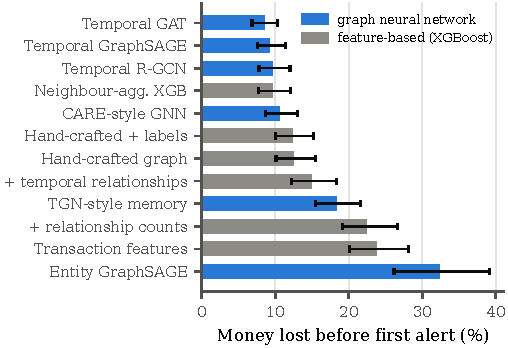
\includegraphics[width=0.49\linewidth]{fig_ringloss.pdf}\hfill
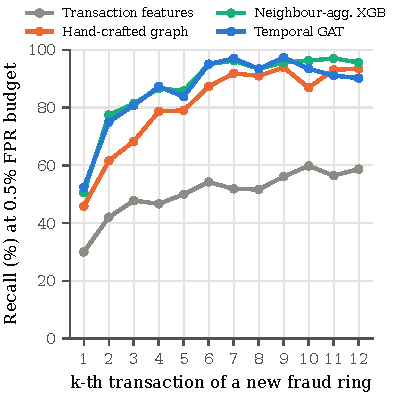
\includegraphics[width=0.49\linewidth]{fig_warmup.pdf}
\caption{Hard preset. Left: ring money lost before the first alert at a 0.1\% alert budget (ring-clustered 95\% CIs). Right: recall on the $k$-th transaction of new rings (0.5\% budget).}\label{fig:ring}
\end{figure}

\textbf{The price of context.} Context also creates false positives on legitimately shared infrastructure: at the 0.5\% budget the Temporal GAT alerts 1.17\% of public Wi-Fi traffic versus 0.17\% of residential traffic, while hand-crafted features stay flat (0.08\% vs.\ 0.24\%).

\subsection{Takedown-Value Weighting}\label{sec:res-tvw}

\begin{table}[!htbp]
\centering
\caption{TVW ($\beta=1$) vs.\ ordinary training of the same model, hyper-parameters and seed (0.5\% budget): money lost before the first alert, paired difference with ring-clustered 95\% CI (bold: excludes 0), and $\Delta$PR-AUC. Simulator: 10 seeds; real data: 3.}\label{tab:tvw}
\footnotesize
\begin{tabular}{@{}lcccc@{}}
\toprule
 & \multicolumn{2}{c}{Money lost (\%)} & & $\Delta$PR-AUC \\
\cmidrule(lr){2-3}
Model & ordinary & TVW & $\Delta$ pp [95\% CI] & (pp) \\
\midrule
\multicolumn{5}{@{}l}{\emph{synthetic (hard)} (322 rings)} \\
Hand-crafted graph features & 7.9 & 6.2 & \textbf{-1.75 [-2.90, -0.83]} & -0.1 \\
\quad + delayed labels & 7.3 & 6.4 & \textbf{-0.87 [-1.56, -0.29]} & -0.1 \\
Neighbour-aggregation XGBoost & 5.2 & 3.9 & \textbf{-1.20 [-2.12, -0.47]} & -0.1 \\
Temporal GraphSAGE & 4.4 & 3.8 & \textbf{-0.58 [-1.14, -0.04]} & -0.4 \\
Temporal GAT & 4.4 & 4.0 & -0.40 [-1.07, +0.28] & -0.2 \\
Temporal CARE-style GNN & 5.2 & 4.2 & \textbf{-1.02 [-1.81, -0.25]} & -0.4 \\
\midrule
\multicolumn{5}{@{}l}{\emph{AMLworld} (84 rings)} \\
Hand-crafted graph features & 0.1 & 0.1 & +0.01 [-0.10, +0.15] & +0.7 \\
\quad + delayed labels & 0.1 & 0.2 & +0.05 [+0.01, +0.16] & -2.6 \\
Neighbour-aggregation XGBoost & 0.0 & 0.0 & +0.00 [-0.02, +0.02] & -1.6 \\
\midrule
\multicolumn{5}{@{}l}{\emph{IEEE-CIS} (675 rings)} \\
Vesta features & 56.2 & 56.5 & +0.26 [-2.90, +3.45] & -0.3 \\
Vesta + hand-crafted graph & 56.9 & 56.8 & -0.03 [-5.27, +6.26] & -0.2 \\
Vesta + graph + delayed labels & 57.4 & 58.1 & +0.74 [-3.55, +5.63] & -0.4 \\
\bottomrule
\end{tabular}

\end{table}

Table~\ref{tab:tvw} and Fig.~\ref{fig:tvw} report TVW for every model and dataset. On the hard preset TVW reduces the money rings take before their first alert for every detector: by 22\% for hand-crafted graph features ($-1.75$ points, CI $[-2.90,-0.83]$) and 25\% for neighbour-aggregation XGBoost, and by 9--20\% for the temporal GNNs at the 0.5\% budget (significant for GraphSAGE and the CARE-style GNN) and 19--25\% at the 1\% budget (significant for all three). The mechanism is visible in first-transaction recall, which rises by 3--8 points for every model (5--7 points for the GNNs), while PR-AUC changes by at most 0.5 points. Pseudo-rings perform as well as true ring labels. On the default preset, where ring losses are already 1--2\%, gains are small (0.2--1.1 points; not shown). On real data the picture is mixed. IEEE-CIS proxy rings are mostly short single-client bursts (median one transaction); there, tempered TVW leaves ring losses unchanged (all CIs include 0) at a PR-AUC cost of only 0.2--0.4 points, whereas the untempered weights reduce ring losses for Vesta + graph features ($-4.6$ points, CI $[-7.7,-1.5]$) but cost 2.4 PR-AUC points: $\gamma$ trades ring-level value against row-level accuracy. On AMLworld, untempered weights collapse onto four transactions (PR-AUC 0.38 $\to$ 0.13), validation selection of $\beta$ falls back to ordinary training, and with ESS tempering PR-AUC stays within $-2.6$ to $+0.7$ points of ordinary training; ring losses change by at most 0.05 points because the relational models already lose only 0.01--0.14\% of pattern money there, leaving no room for improvement. TVW therefore helps where early-ring losses exist and is safe where they do not.


\begin{figure}[!htbp]
\centering
\begin{minipage}[t]{0.49\linewidth}\centering
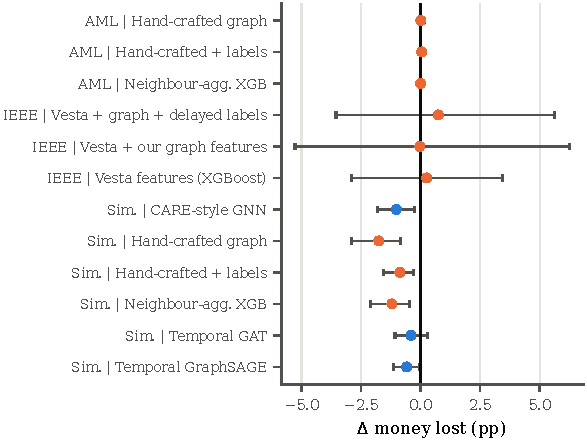
\includegraphics[width=\linewidth]{fig_tvw.pdf}
\caption{Effect of TVW on ring money lost before the first alert (0.5\% budget; negative is better; 95\% ring-clustered CIs). Blue: GNNs; orange: feature-based models.}\label{fig:tvw}
\end{minipage}\hfill
\begin{minipage}[t]{0.49\linewidth}\centering
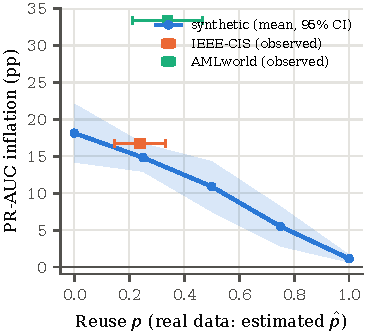
\includegraphics[width=\linewidth]{fig_leakage.pdf}
\caption{PR-AUC inflation of the transductive protocol vs.\ attacker infrastructure reuse (simulator, 5 seeds) and on real data at its estimated reuse level $\hat p$.}\label{fig:leak}
\end{minipage}
\end{figure}

\subsection{When Context Helps and When Evaluations Mislead}\label{sec:res-context}

\begin{table}[!htbp]
\centering
\caption{Real data: test PR-AUC, mean $\pm$ s.d.\ over 3 seeds (IEEE-CIS also on each client's first fraud transaction). AMLworld temporal GNNs are trained on all laundering plus a 30\% sample of legitimate transfers; Vesta features exist only for IEEE-CIS (n/a). $^\dagger$Leaky transductive protocol, shown for contrast only.}\label{tab:real}
\footnotesize
\begin{tabular}{@{}lccc@{}}
\toprule
 & AMLworld & \multicolumn{2}{c}{IEEE-CIS} \\
\cmidrule(lr){2-2}\cmidrule(lr){3-4}
Model & PR-AUC & PR-AUC & PR-AUC (1st fraud) \\
\midrule
Transaction features & 0.130\,$\pm$\,0.009 & 0.134\,$\pm$\,0.003 & 0.058\,$\pm$\,0.001 \\
Hand-crafted graph features & 0.377\,$\pm$\,0.015 & 0.186\,$\pm$\,0.006 & 0.097\,$\pm$\,0.005 \\
\quad + delayed labels & 0.480\,$\pm$\,0.010 & 0.404\,$\pm$\,0.002 & 0.114\,$\pm$\,0.001 \\
Neighbour-aggregation XGBoost & 0.539\,$\pm$\,0.005 & 0.218\,$\pm$\,0.004 & 0.117\,$\pm$\,0.001 \\
Temporal GraphSAGE & 0.470\,$\pm$\,0.007 & 0.224\,$\pm$\,0.006 & 0.132\,$\pm$\,0.009 \\
Temporal GAT & 0.465\,$\pm$\,0.004 & 0.204\,$\pm$\,0.010 & 0.107\,$\pm$\,0.010 \\
\midrule
Entity GraphSAGE (inductive) & 0.004\,$\pm$\,0.000 & 0.082\,$\pm$\,0.014 & 0.046\,$\pm$\,0.009 \\
Entity GraphSAGE (transductive)$^\dagger$ & 0.338\,$\pm$\,0.033 & 0.249\,$\pm$\,0.012 & 0.103\,$\pm$\,0.011 \\
\midrule
Vesta features & n/a & 0.536\,$\pm$\,0.004 & 0.472\,$\pm$\,0.002 \\
Vesta + hand-crafted graph & n/a & 0.535\,$\pm$\,0.003 & 0.471\,$\pm$\,0.004 \\
Vesta + graph + delayed labels & n/a & 0.621\,$\pm$\,0.004 & 0.454\,$\pm$\,0.006 \\
\bottomrule
\end{tabular}

\end{table}

\textbf{Real data.} On AMLworld (Table~\ref{tab:real}), relational context raises PR-AUC from 0.130 with transaction features to 0.377 with hand-crafted graph features and 0.539 with neighbour-aggregation XGBoost, and on the 28 ground-truth patterns that start in the test window, transaction features let 44\% of pattern money through before the first alert against 0.1--0.8\% for the full hand-crafted graph features, neighbour aggregation and the temporal GNNs (0.1\% budget). The temporal GNNs, trained on all laundering plus a 30\% sample of legitimate transfers because of the 5.08M-row scale, reach 0.470 (GraphSAGE) and 0.465 (GAT), nine points above hand-crafted graph features and stable across seeds ($\pm$0.007), and lose only 0.4\% of pattern money before the first alert; neighbour-aggregation XGBoost remains the strongest model at this prevalence (0.09\%). On IEEE-CIS, relational context and temporal GNNs clearly improve transaction features, including on first-fraud transactions (0.058 $\to$ 0.132 for Temporal GraphSAGE), but add nothing on top of Vesta's engineered features (0.535 vs.\ 0.536), which already encode relational counts: the value of context depends on what the feature store already contains. A temporal GAT over Vesta's 430 heterogeneous features also stays below the tree model (0.437), as neural networks commonly do on wide tabular data.

\begin{table}[!htbp]
\centering
\caption{PR-AUC gain (points, mean $\pm$ 95\% CI over 5 seeds) from delayed neighbour-label features, by label delay $D$ and ring lifetime (simulator, fresh infrastructure per ring). Bold: CI excludes 0.}\label{tab:delay}
\small
\begin{tabular}{@{}lccccc@{}}
\toprule
Ring lifetime & $D$\,=\,0\,d & $D$\,=\,1\,d & $D$\,=\,7\,d & $D$\,=\,30\,d & $D$\,=\,90\,d \\
\midrule
1-3 d & \textbf{+0.42\,$\pm$\,0.21} & -0.00\,$\pm$\,0.12 & +0.00\,$\pm$\,0.07 & -0.02\,$\pm$\,0.07 & -0.03\,$\pm$\,0.06 \\
7-14 d & \textbf{+0.98\,$\pm$\,0.65} & +0.44\,$\pm$\,0.45 & +0.12\,$\pm$\,0.13 & -0.03\,$\pm$\,0.12 & -0.05\,$\pm$\,0.09 \\
30-60 d & \textbf{+2.65\,$\pm$\,0.47} & \textbf{+2.33\,$\pm$\,0.50} & \textbf{+1.89\,$\pm$\,0.55} & \textbf{+0.28\,$\pm$\,0.23} & +0.02\,$\pm$\,0.10 \\
60-120 d & \textbf{+4.09\,$\pm$\,0.97} & \textbf{+3.86\,$\pm$\,0.94} & \textbf{+3.37\,$\pm$\,0.92} & \textbf{+0.98\,$\pm$\,0.53} & +0.06\,$\pm$\,0.08 \\
\bottomrule
\end{tabular}

\end{table}

\textbf{Label delay versus ring lifetime.} Neighbour-label features (``this device was used in confirmed fraud'') are among the strongest signals in practice, but labels arrive late. Table~\ref{tab:delay} shows that they help only while the delay is shorter than the ring's lifetime: for rings living 1--3 days the gain vanishes at a one-day delay, whereas rings living 60--120 days still gain 1 point at $D=30$ days. AMLworld's ground-truth patterns behave the same way: PR-AUC falls from 0.510 with instant labels to 0.360 without labels as the delay grows, tracking a model-free \emph{reachability} statistic---the share of test laundering whose pattern has a matured label---that drops from 0.54 to 0. On IEEE-CIS, by contrast, the apparent +8.5-point gain from 30-day-delayed labels is an artefact of the client-level labelling convention: on first-fraud transactions the labels \emph{reduce} PR-AUC by 1.8 points.

\textbf{Transductive evaluation inflates results.} Many GNN fraud studies build one graph over all transactions, including test ones. Varying attacker infrastructure reuse $p$ in the simulator, this transductive protocol inflates PR-AUC by 18.1 points when every ring uses fresh infrastructure ($p=0$) but only 1.2 points when rings reuse a fixed pool ($p=1$) (Fig.~\ref{fig:leak})---so benchmarks with persistent attackers hide the leak. Ignoring label delay adds a further 1.1 points, while random splits showed no detectable effect once compared on the same rows. The share of test fraud on entities already used by fraud in training is 15--16\% on IEEE-CIS, which places it at $\hat p=0.15$--$0.33$ on the simulator's dial. At that $\hat p$ the simulator predicts 13.6--16.2 points of transductive inflation; IEEE-CIS shows 16.7 (0.249 vs.\ 0.082). On AMLworld ($\hat p=0.21$--$0.47$) the observed inflation is far larger, +33 points (0.338 vs.\ 0.004), than the 11--15 points predicted: the simulator gets the direction right but underestimates the magnitude at AMLworld's 40$\times$ lower fraud prevalence, consistent with our sensitivity sweep, where inflation grew to +45 points at a 1\% fraud rate. Part of the AMLworld gap, however, reflects a weak inductive baseline: the entity GraphSAGE uses unsupervised embeddings only, and its count-based node features shift when applied to the larger test-time history graph, so IEEE-CIS gives the cleaner estimate.


%=====================================================================
\section{Discussion and Limitations}
%=====================================================================
Context-aware GNNs are worth their cost mainly because they catch rings \emph{earlier}, a benefit row-level metrics understate; training on the ring's clock adds to it on the simulator, while on real data its value depends on how much early-ring structure the labels expose. Limitations: first, simulator magnitudes depend on its assumptions (mitigated by the hard preset, a sensitivity sweep and two real datasets). Second, no public dataset combines real transactions with ground-truth rings: IEEE-CIS rings are proxies and AMLworld is itself simulated. Third, context creates disparate false-positive rates on shared infrastructure, which we measure but do not solve. Finally, a greedy black-box attacker needed 6--7$\times$ its normal resources to evade relational detectors versus 2.5$\times$ for transaction features, mostly through ``slow-and-low'' operation.

%=====================================================================
\section{Conclusion}
%=====================================================================
We evaluated context-aware fraud detection on the ring's clock. Temporal GNNs over a strictly-past neighbourhood reduce the money a ring takes before its first alert by 41--45\% relative to hand-crafted graph features, and takedown-value weighting, a ring-level training objective that needs no ring labels, reduces it by a further 9--25\% across architectures on the simulator and is neutral on real data, where early-ring losses are already small. We also showed when relational context helps (label delay shorter than ring lifetime) and how much leaky protocols inflate reported results. We release the simulator and evaluation code to encourage reporting fraud detection on the clock that matters.

\bibliographystyle{vancouver}
\bibliography{refs}

\end{document}
